\documentclass[aps,reprint,prl,floatfix,nofootinbib]{revtex4-1}
\usepackage{graphicx}  % needed for figures
\usepackage{bm}        % for math
\usepackage{amsmath,amssymb}   % for math
\usepackage{url}
\usepackage{hyperref,float}
\restylefloat{figure}
%\usepackage{notoccite}

\begin{document}
\title{An Exploration of the Friedmann Equations}
\author{Steven M. Kaplan}
\affiliation{Department of Physics and Astronomy, Rutgers, The State University of New Jersey, 136 Frelinghuysen Road, Piscataway, New Jersey 08854, USA}

\begin{abstract}
The Friedmann equations are very powerful tools in cosmology.  Given the densities $\rho$ of matter, radiation, and dark energy, one can solve the Friedmann equations to obtain the scale factor $a(t)$, the measure of how much the universe has expanded at a given moment relative to the present time which, by convention, is assigned a scale factor of unity.  Once $a(t)$ is known, other quantities can be obtained such as the age of the universe in the model and the time evolution of the Hubble constant.  The above is explored using six cosmological models followed by a discussion of which models predict an 'end' of the universe and which predict an infinitely long expansion period.
\end{abstract}

\maketitle

\section*{Introduction}
The assumption of a homogeneous and isotropic universe, collectively known as the cosmological principle \cite{cosmoprinciple}, gives rise to the Friedmann-Robertson-Walker (FRW) metric:
$$ds^2=-dt^2 + a(t)^2\left[ \frac{dr^2}{1-kr^2} + r^2d\Omega^2 \right]$$
If the model universe is expanding (or contracting), the physical distance between any two objects changes over time.  This motivates the idea of \emph{comoving distance}, which by construction keeps the distance between the two objects constant.  The scale factor a(t) seen in the FRW metric is the ratio of the physical distance to the comoving distance \cite{wiki_scalefactor}.  If $a(t)$ increases over time, then the universe is expanding.  Conversely, if $a(t)$ decreases over time, then the universe is detracting.  The parameter $k$ describes the overall curvature of the universe and can take on the values $0,\pm1$.

An in-depth discussion of the derivation of the Friedmann equations can be found in many sources, the most helpful to the author being \cite{carroll}.  The stress-energy tensor is assumed to be that of a perfect fluid:
$$T^{\mu}_{\nu}=diag(-\rho,P,P,P)$$
Using the $00$ component of the Einstein field equation
$$R_{\mu\nu}-\frac{1}{2}g_{\mu\nu}R=8\pi GT_{\mu\nu} $$
in conjunction with the stress energy tensor above leads to one of the Friedmann equations:
\begin{equation}
\left(\frac{\dot{a}}{a}\right)^2=\frac{8\pi G}{3}\rho-\frac{k}{a^2}
\end{equation}
Here, $\rho=\rho(t)=\rho_{m}(t)+\rho_{r}(t)+\rho_{DE}(t)$
where the subscripts $m$, $r$, and $DE$ stand for matter, radiation, and dark energy, respectively.  From the conservation of the energy-momentum tensor and the fact that the equation of state obeys $P=w\rho$, the following relation is obtained:
$$\frac{ \dot{\rho} }{\rho}=-3(1+w)\frac{ \dot{a} }{a}$$
This yields the solution
\begin{equation}
\rho=\rho_0a^{-3(1+w)}
\end{equation}
where
\[w = \left\{
  \begin{array}{lr}
    0 & matter\\
    \frac{1}{3} & radiation\\
    -1 & dark\;energy
  \end{array}
\right.
\]
The quantity $\rho_0$ is the energy density today with the condition that $a(today)=1$.  In this paper, the densities will be expressed in terms of the density parameter 
$$\Omega_x \equiv \frac{ \rho_{x} }{\rho_{cr}}$$
with $x$ representing one of matter, radiation, and dark energy.  The critical density is defined to be
$$\rho_{cr}=\frac{3H^2}{8\pi G}\;.$$
It is termed the critical density as it can be thought of as the crossover point between a universe being open or closed.  The Hubble parameter
\begin{equation} \label{eq:hubble}
H\equiv \frac{ \dot{a} }{a}
\end{equation}
represents the rate of the expansion of the universe.  This paper will assume that the Hubble parameter today
$$H_0=70\;\frac{km}{s\cdot Mpc}=7.16\cdot10^{-2}\;Gyr$$
Using the fact that $\rho_0=\Omega_0 \rho_{cr}$ and explicitly showing the $a$ dependence of the densities, the Friedmann equation can be written in a form more easily usable for the purpose of this paper:
\begin{equation} \label{eq:friedmann}
\left(\frac{\dot{a}}{a}\right)^2=H_0^2\left[ \frac{\Omega_{m,0}}{a^3}+\frac{\Omega_{r,0}}{a^4}+\frac{\Omega_{DE,0}}{a^{3(1+w)}} \right] -\frac{k}{a^2}
\end{equation}
\newpage
This paper discusses the solution of equation \ref{eq:friedmann} in the following cases (if not specified, a quantity should be assumed to be equal to zero):
\begin{itemize}
\item $\Omega_{m,0}=1$ (Einstein-de Sitter Universe)
\item $\Omega_{m,0}=2,\;k=1$ (Closed Universe)
\item $\Omega_{m,0}=0.3,\;k=-1$ (Open Universe)
\item $\Omega_{m,0}=0.3,\;\Omega_{DE,0}=0.7,\;w=-1$ ($\Lambda_{CDM}$)
\item $\Omega_{m,0}=0.3,\Omega_{DE,0}=0.7,w=-2/3$ (Quintessence)
\item $\Omega_{m,0}=0.3,\Omega_{DE,0}=0.7,w=-4/3$ (Phantom Energy)
\end{itemize}
Note that since recent measurements \cite{pdg} of \\$\Omega_{r,0}=2.47\cdot10^{-5}h^{-2}$, its contribution to the scale factor is negligible given the time scale considered.
\section*{Method}
To solve equation \ref{eq:friedmann} numerically and to fit the solutions, the \texttt{SciPy} library \cite{scipy} was used.  In order to avoid divergences as $a\rightarrow0$, the value of $t$ was defined relative to the present.  The present day value of the scale factor was set to unity.  Were this not the case and since there is no explicit $t$ dependence in the Friedmann equation, the form of $a(t)$ would simply be shifted; however, the shape would remain the same.  A change in the setting of the scale factor today would not alter $H(t)$ since any change to the scale factor would cancel.  To plot $a(t)$ and $H(t)$, the \texttt{PyROOT} wrapper of the \texttt{ROOT} data analysis library \cite{ROOT} was used.  Using the fit for $a(t)$, one can use equation \ref{eq:hubble} to visualize the time evolution of the Hubble constant.  By the definition of the scale factor, the big bang occurred at the value of $t$ where $a(t) = 0$.
\section*{Results}
The solutions $a(t)$ from solving equation \ref{eq:friedmann} numerically for each model of the universe is shown in Figure 1, and the corresponding Hubble parameter given by equation \ref{eq:hubble} is shown in Figure 2.

\begin{figure}[H]
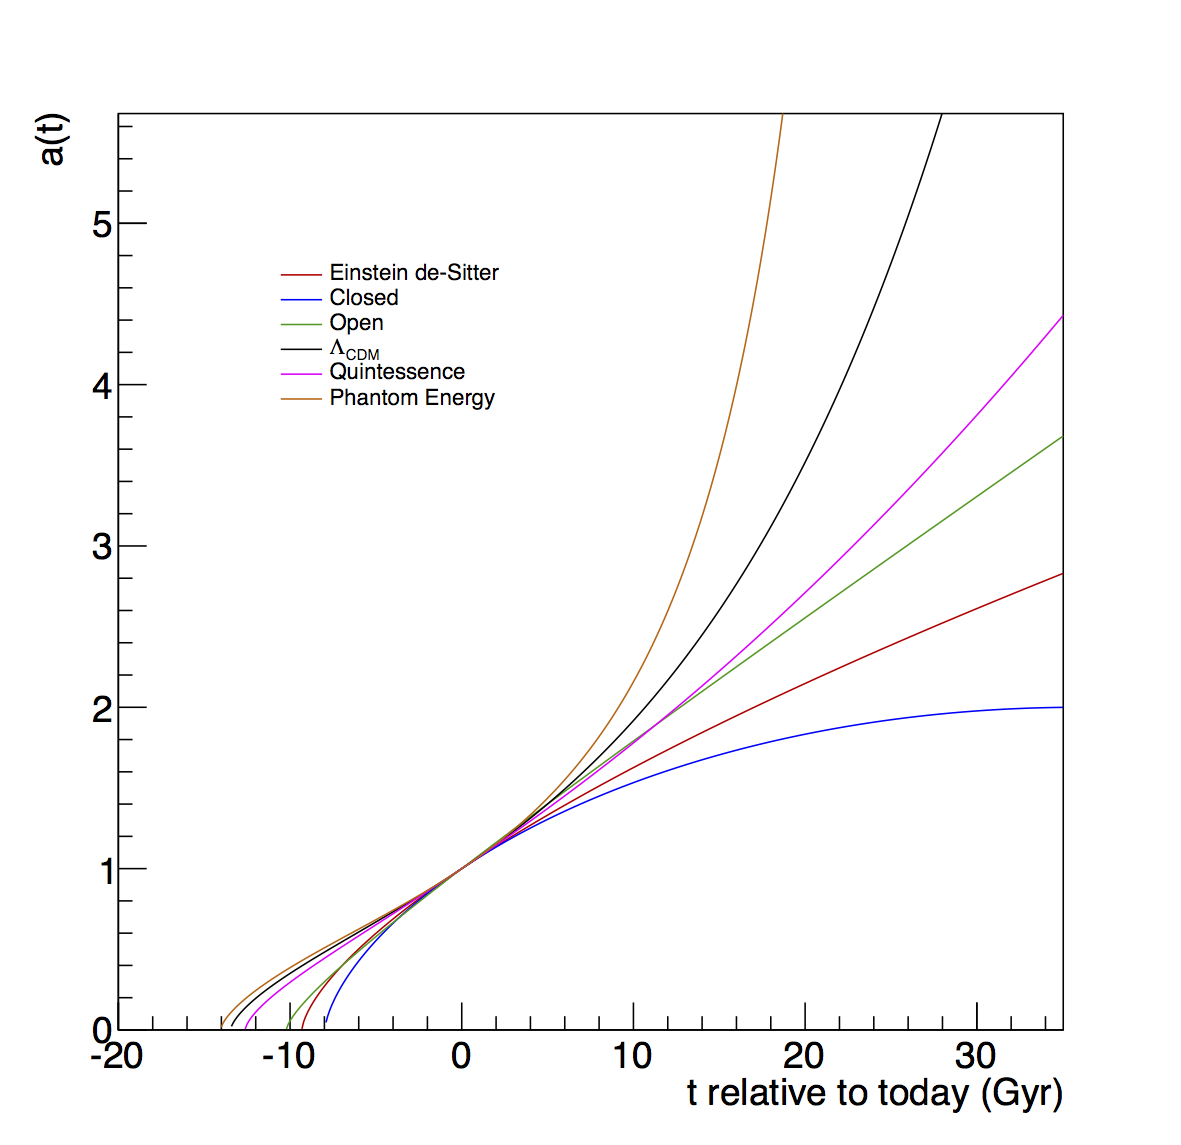
\includegraphics[width=0.5\textwidth]{ps1_plots/a1-6}
\caption{The time evolution of the scale factor $a(t)$}
\end{figure}

Each plot was fit with the function $a(t)=k(t-t_0)^n$ save for the phantom energy case for which this fit was unreasonable, and the author was unable to find a better fit function.  Instead, in order to get $\dot{a}(t)$, the slope in between each point in $a(t)$ is used.  As mentioned above, the big bang will have occurred at the value of $t$ for which $a(t) = 0$.  This corresponds to the value of $t_0$ in the fit.\\

\begin{figure}[H]
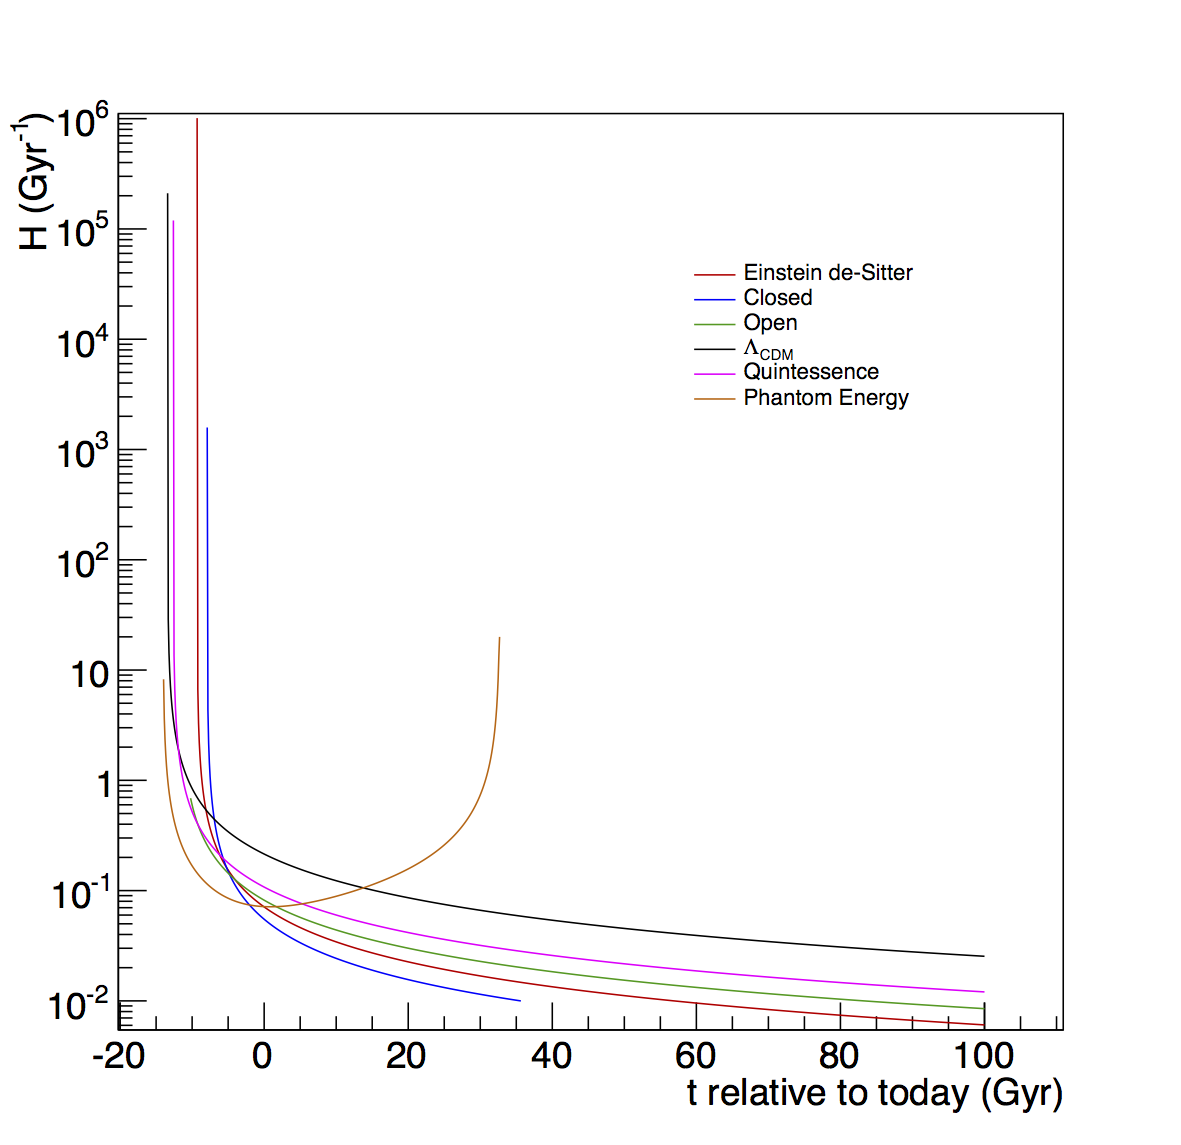
\includegraphics[width=0.5\textwidth]{ps1_plots/h1-6}
\caption{The time evolution of the Hubble paramter $H(t)$}
\end{figure}
\newpage
\begin{table}[h]
\begin{tabular}{c|c|c|c}
Model              & $k$    & $t_0$ (Gyr) & $n$    \\
                   &        &             &        \\ \hline
Einstein-de Sitter & 0.2305 & 9.309       & 0.6618 \\ \hline
Closed             & 0.4179 & 7.908       & 0.4349 \\ \hline
Open               & 0.0964 & 11.59       & 0.9483 \\ \hline
$\Lambda_{CDM}$    & 0.0003 & 13.41       & 2.878  \\ \hline
Quintessence       & 0.0254 & 12.61       & 1.358  \\ \hline
Phantom Energy     & N/A    & $\sim$15    & N/A   
\end{tabular}
\caption{Fit parameters for the cosmological models considered.  Note that for the phantom energy model, the age of the universe quoted is based on a qualitative look at the solution for $a(t)$ only.}
\end{table}
There are a number of interesting results (see Table 1) to discuss here.  First, according to the fits, the Einstein de-Sitter and closed universes would not be consistent with the measured age of globular clusters $(13\pm2$ Gyr).  Also, the closed universe model predicts a big crunch (\emph{i.e.} the universe will not expand indefinitely but will contract in a finite amount of time) at $\sim$70 Gyr.  Of particular interest to the author is that the phantom energy model predicts a big rip (\emph{i.e.} the universe will come to expand at an infinite rate within a finite amount of time) at $\sim$32 Gyr.  A curious outcome of this model is that the Hubble parameter does not decrease monotonically.  Since we expect the age of the universe to be proportional to $\frac{1}{H}$, $H$ should thus be expected to decrease monotonically for the age of the universe to increase over time.  As can be seen in Figure 2, $H(t)$ increases over much of the universe's existence.  Quite dramatically, as is described in \cite{Caldwell:2003vq}, the big rip would unbind our solar system on the order of months and destroy the earth on the order of minutes before the universe meets its fate.


\bibliographystyle{unsrt}
\bibliography{ps1Sources}

%\begin{thebibliography}{99}
%
%\bibitem{wiki_scalefactor}
%Wikipedia contributors, "Scale factor (cosmology)," Wikipedia, The Free Encyclopedia, \url{http://en.wikipedia.org/w/index.php?title=Scale_factor_(cosmology)&oldid=642845167} (accessed February 11, 2015).
%
%\bibitem{carroll}
%Sean Carroll, Lecture Notes on General Relativity, \url{http://preposterousuniverse.com/grnotes/} (accessed February 11, 2015)
%
%\bibitem{scipy}
%Jones E, Oliphant E, Peterson P, et al. SciPy: Open Source Scientific Tools for Python, 2001-, \url{http://www.scipy.org/} 
%
%\bibitem{ROOT}
%Rene Brun and Fons Rademakers, ROOT - An Object Oriented Data Analysis Framework, Proceedings AIHENP'96 Workshop, Lausanne, Sep. 1996, Nucl. Inst. \& Meth. in Phys. Res. A 389 (1997) 81-86. See also \url{http://root.cern.ch/}.
%
%\end{thebibliography}

\end{document}